\documentclass[11pt]{article}
\usepackage[margin=1in]{geometry}
\usepackage{amsmath,amssymb,booktabs,array,longtable}
\usepackage{graphicx}
\usepackage{hyperref}
\usepackage{enumitem}
\usepackage{titlesec}
\usepackage{float}

\begin{document}

\begin{center}
\Large\textbf{Shiv Nadar University Chennai}\\[2mm]
\end{center}

\renewcommand{\arraystretch}{1.4}

\begin{tabular}{|p{3.5cm}|p{8cm}|p{2cm}|}
\hline
Degree \& Branch & B.Tech Artificial Intelligence \& Data Science & Semester V\\ \hline
Subject Code \& Name & CS3807 -- Deep Learning Laboratory & AY: 2026--27\\ \hline
\end{tabular}

Name : Ashwin S\\
Reg no : 24011101007\\
Class : AI DS - A (batch 1)\\

\vspace{3mm}

\begin{center}
\Large\textbf{Experiment 1}\\
\large\textbf{Implementation of a Single Layer Perceptron for Binary Classification}
\end{center}

%----------------------------------------------------------

\section*{1. Objective}

The objective of this experiment is to understand the concept of an artificial neuron and implement a Single Layer Perceptron from scratch for binary classification. The perceptron learning algorithm is implemented without relying on high-level machine learning libraries, the role of the activation function is studied, the learning process is visualized across epochs, and the classifier is evaluated on a real-world dataset using standard performance metrics.

%----------------------------------------------------------

\section*{2. Tasks Performed}

\begin{enumerate}[leftmargin=*]
\item Downloaded and understood the dataset.
\item Performed Exploratory Data Analysis (EDA).
\item Preprocessed the dataset (standardization, train/test split).
\item Implemented a Single Layer Perceptron from scratch using NumPy.
\item Trained the model using the perceptron learning rule.
\item Evaluated the classifier using standard performance metrics.
\item Analyzed the effect of different learning rates.
\item Compared the implementation with Scikit-learn's Perceptron.
\end{enumerate}

%----------------------------------------------------------

\section*{3. Background Theory}

An Artificial Neuron is the fundamental building block of a neural network. It receives one or more input features, multiplies them by corresponding weights, adds a bias term, and applies an activation function to determine the output.

The Single Layer Perceptron is the earliest supervised learning algorithm capable of solving linearly separable binary classification problems.

\subsection*{Mathematical Formulation}

Weighted Sum

\[
z=\mathbf{w}^{T}\mathbf{x}+b
\]

where

\begin{itemize}
\item $\mathbf{x}$ : Input vector
\item $\mathbf{w}$ : Weight vector
\item $b$ : Bias
\item $z$ : Linear combination
\end{itemize}

Prediction

\[
\hat y=f(z)
\]

Weight Update Rule

\[
\mathbf{w}_{new}
=
\mathbf{w}_{old}
+
\eta
(y-\hat y)
\mathbf{x}
\]

Bias Update

\[
b_{new}
=
b_{old}
+
\eta
(y-\hat y)
\]

where $\eta$ denotes the learning rate.

In this implementation, weights were initialized from a small Gaussian distribution ($\mathcal{N}(0, 0.01^2)$) rather than zeros, and the bias was initialized to $0$. Updates were performed online -- i.e.\ sample by sample within each epoch -- following the classical Rosenblatt rule shown above.

%----------------------------------------------------------

\section*{4. Activation Functions}

An activation function determines the output of a neuron based on the weighted sum of its inputs. It introduces non-linearity, enabling neural networks to learn complex patterns. Although the perceptron uses only the Step Activation Function, modern deep learning models employ differentiable activation functions for efficient optimization through backpropagation.

\subsection*{Step Activation Function}

\[
f(z)=
\begin{cases}
1,&z\ge0\\
0,&z<0
\end{cases}
\]

The Step Activation Function produces a binary output and is therefore suitable only for linearly separable binary classification problems.

\begin{center}
\begin{tabular}{|p{2.5cm}|p{3cm}|p{6cm}|}
\hline
\textbf{Activation} & \textbf{Output Range} & \textbf{Typical Applications}\\
\hline
Step & $\{0,1\}$ & Classical Perceptron\\
\hline
Sigmoid & $(0,1)$ & Binary Classification Output Layer\\
\hline
Tanh & $(-1,1)$ & Hidden Layers (Traditional Networks)\\
\hline
ReLU & $[0,\infty)$ & Hidden Layers in CNNs and MLPs\\
\hline
Leaky ReLU & $(-\infty,\infty)$ & Avoiding Dying ReLU\\
\hline
Softmax & $(0,1)$ & Multi-class Classification Output Layer\\
\hline
\end{tabular}
\end{center}

\textbf{Note:} This experiment uses only the Step Activation Function. The remaining activation functions will be studied in subsequent experiments involving Multilayer Perceptrons and Deep Neural Networks.

%----------------------------------------------------------

\section*{5. Dataset Description}

\textbf{Dataset:} Banknote Authentication Dataset

\textbf{Source:} UCI Machine Learning Repository

\textbf{Download Link:}

\url{https://archive.ics.uci.edu/dataset/267/banknote+authentication}

\begin{center}
\begin{tabular}{|l|l|}
\hline
Instances & 1372\\
\hline
Features & 4 Numerical Features\\
\hline
Classes & 2\\
\hline
Missing Values & None\\
\hline
Task & Binary Classification\\
\hline
\end{tabular}
\end{center}

\textbf{Feature Description}

\begin{itemize}
\item Variance
\item Skewness
\item Curtosis
\item Entropy
\end{itemize}

Target Class

\begin{itemize}
\item 0 -- Authentic Banknote
\item 1 -- Forged Banknote
\end{itemize}

%----------------------------------------------------------

\section*{6. Experimental Procedure}

\textbf{Task 1: Dataset Exploration}
\begin{itemize}
\item Load the dataset.
\item Display the first five samples.
\item Determine dataset dimensions.
\item Identify missing values.
\item Display descriptive statistics.
\end{itemize}
Expected Output: Dataset summary and statistical information.

\vspace{2mm}

\textbf{Task 2: Exploratory Data Analysis}

Generate
\begin{itemize}
\item Histograms
\item Correlation Heatmap
\item Scatter Plot
\item Boxplots
\end{itemize}

\vspace{2mm}

\textbf{Task 3: Data Preprocessing}
\begin{itemize}
\item Normalize all numerical features.
\item Split the dataset into Training (80\%) and Testing (20\%).
\end{itemize}

\vspace{2mm}

\textbf{Task 4: Perceptron Implementation}

Implement from scratch
\begin{itemize}
\item Weight Initialization
\item Bias Initialization
\item Step Activation Function
\item Forward Propagation
\item Perceptron Learning Rule
\end{itemize}

\vspace{2mm}

\textbf{Task 5: Model Training}

Display
\begin{itemize}
\item Epoch Number
\item Misclassified Samples
\item Updated Weights
\item Updated Bias
\end{itemize}

\vspace{2mm}

\textbf{Task 6: Model Evaluation}

Compute
\begin{itemize}
\item Accuracy
\item Precision
\item Recall
\item F1-score
\item Confusion Matrix
\end{itemize}

%----------------------------------------------------------

\section*{7. Experimental Results}

The single layer perceptron model was trained on the Banknote Authentication dataset for 50 epochs at a learning rate of $\eta = 0.01$. The first epoch misclassified 53 samples, which reduced to just 12 at the end of 50th epoch. The model does not converge within 50 epochs, indicating that the two classes are close to linearly separable but actually is non-linearly separable.

The final weights vector after learning was $[-0.1931,\ -0.2132,\ -0.2176,\ -0.0217]$ (corresponding to variance, skewness, curtosis, and entropy respectively), and the final bias was $-0.1000$. The magnitudes of these weights indicate that variance, skewness, and curtosis contributed most strongly to the decision boundary, while entropy contributed the least.

In the test set of 275 samples, the trained model achieved an accuracy of 97.81\%, a precision of 98.37\%, a recall of 96.80\% and an F1-score of 0.9758. The confusion matrix shows 147 true negatives, 121 true positives, 2 false positives, and 4 false negatives. All learning rates among  $\eta \in \{0.001, 0.01, 0.1\}$  were tested, representing the trade-off between convergence speed and stability, and produced similar results to builtin Perceptron (accuracy of 0.9781). This indicates the correctness of manual implementation.

%----------------------------------------------------------

\section*{8. Mandatory Plots and Interpretations}

All plots were generated in vector \texttt{.eps} format at 600 DPI quality.

\subsection*{8.1 Feature Histograms}
\begin{figure}[H]
\centering
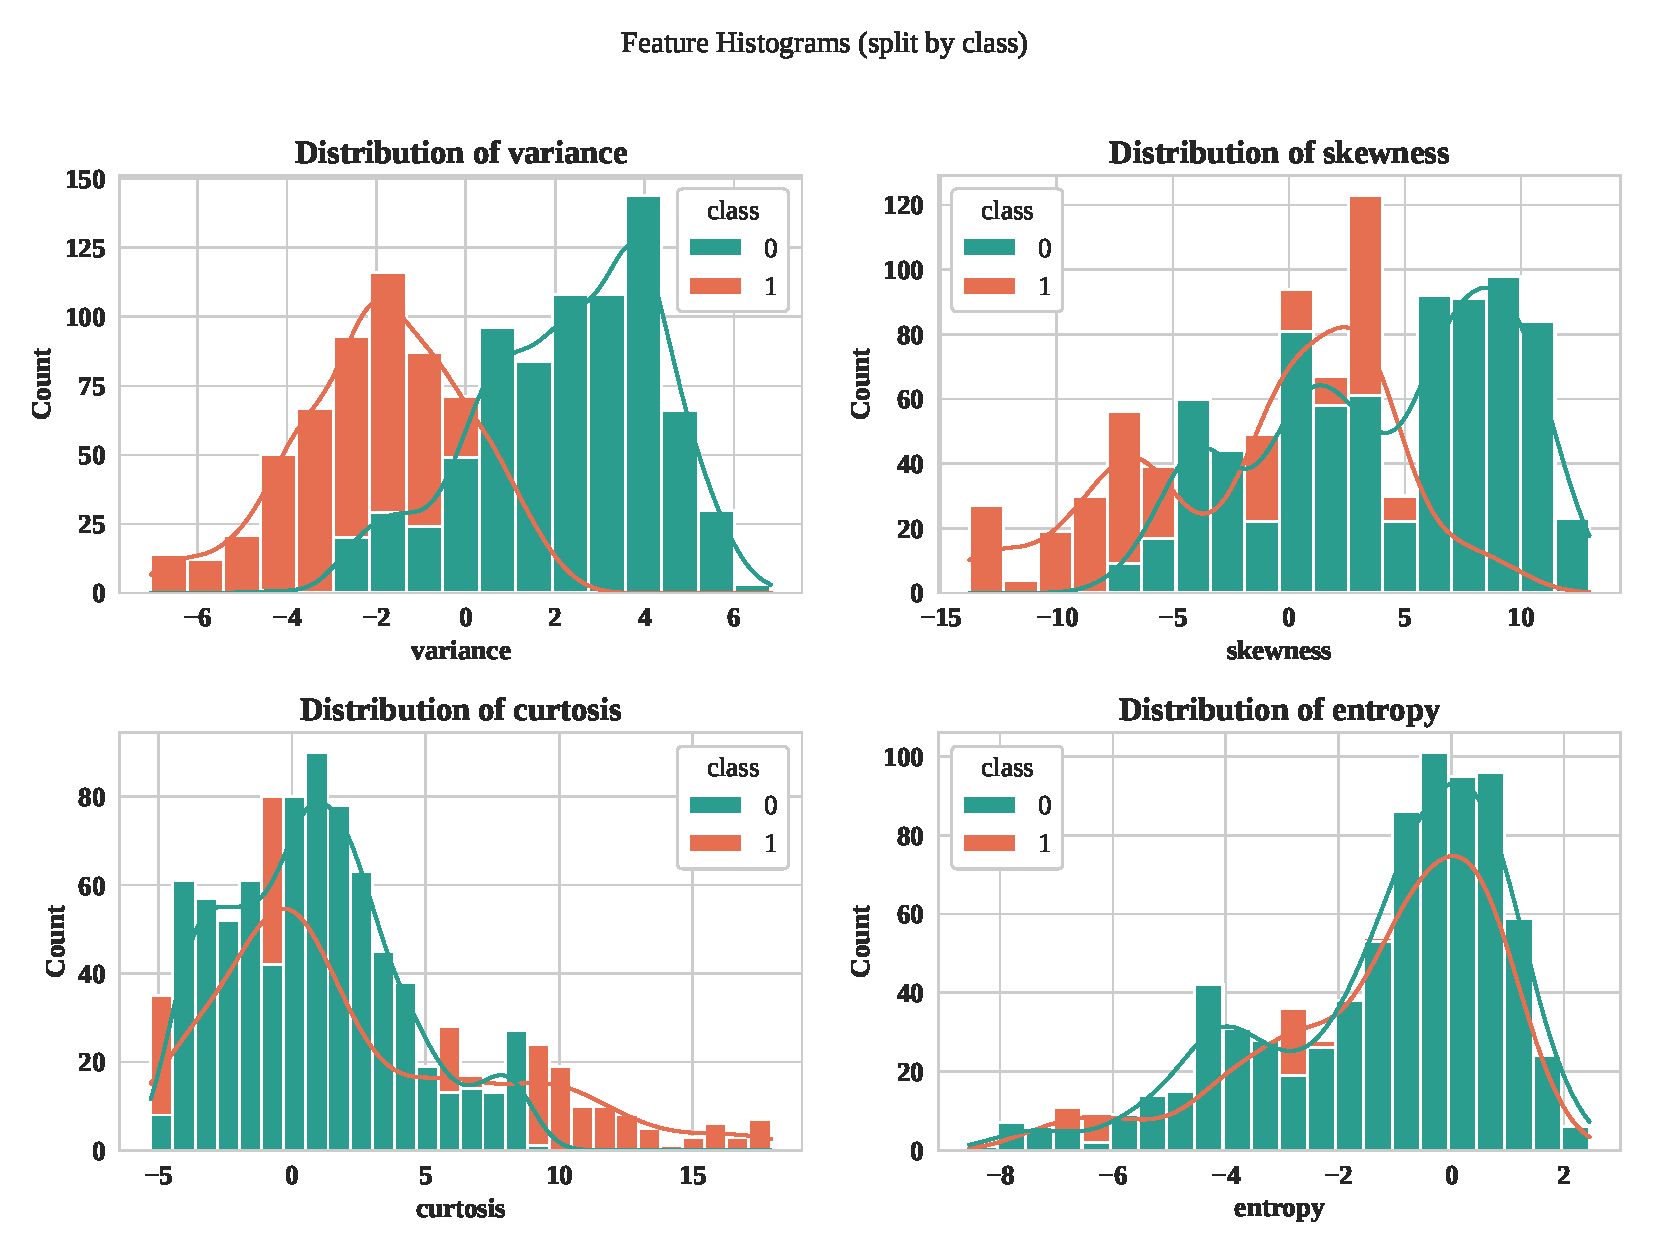
\includegraphics[width=0.85\textwidth]{figures/task2_feature_histograms.eps}
\caption{Distribution of each feature, split by class.}
\end{figure}

Variance shows clearly separated distribution between the two classes. Authentic notes tend to have higher variance, forged notes have lower variance. Entropy shows heavy overlap between classes, making it the weakest differentiating feature. Curtosis shows a long right tail with partial overlap.

\subsection*{8.2 Correlation Heatmap}
\begin{figure}[H]
\centering
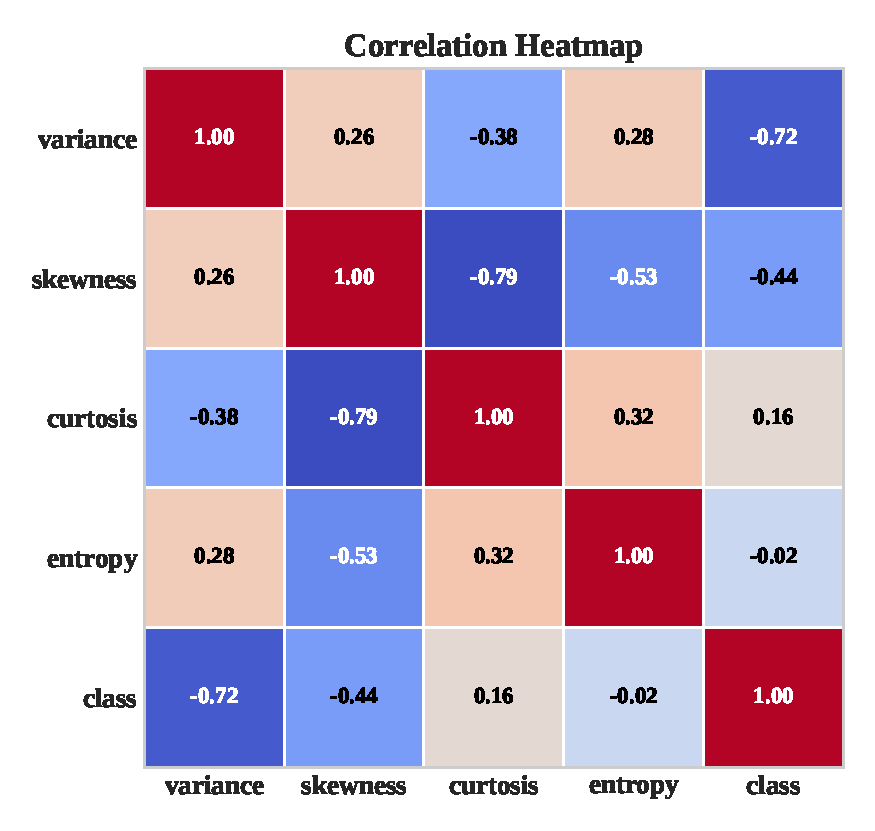
\includegraphics[width=0.6\textwidth]{figures/task2_correlation_heatmap.eps}
\caption{Correlation heatmap of the four features and the class label.}
\end{figure}

Variance has the strongest correlation with class. Skewness and curtosis show moderate correlation with each other, which might be indicating some feature redundancy. Entropy correlates weakly with class, similar to its overlapping in the histogram plot.

\subsection*{8.3 Scatter Plot}
\begin{figure}[H]
\centering
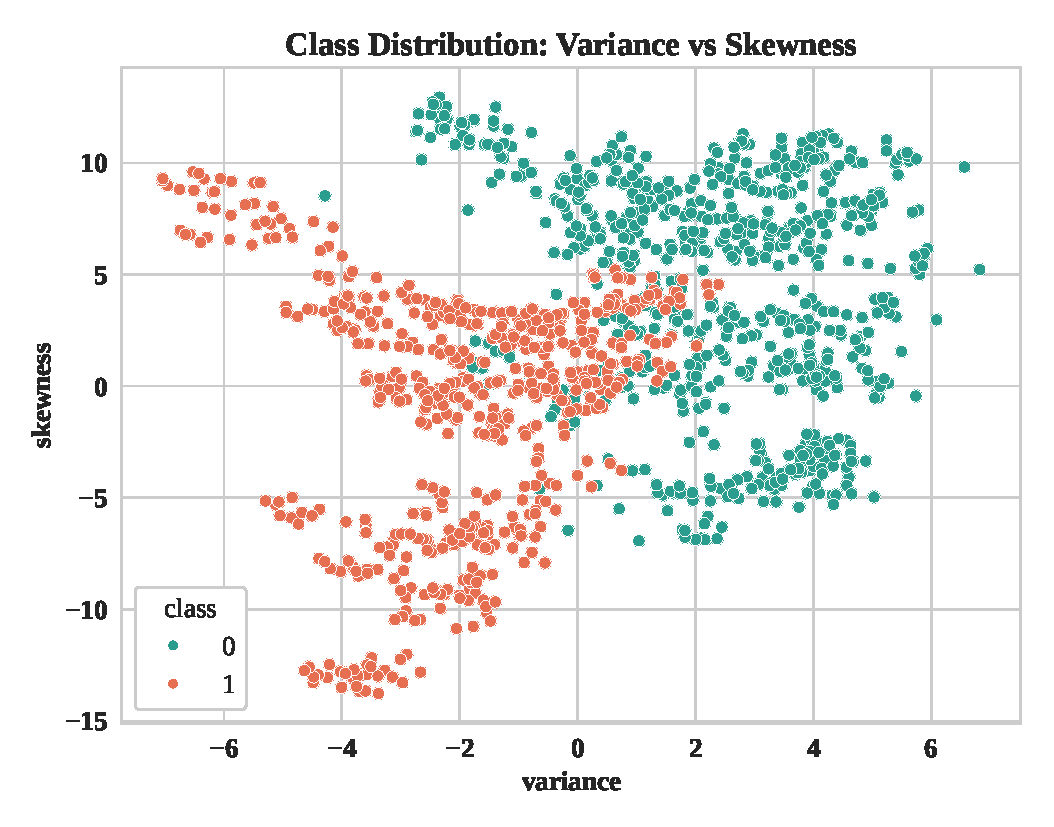
\includegraphics[width=0.6\textwidth]{figures/task2_scatter_variance_skewness.eps}
\caption{Class distribution: variance vs.\ skewness.}
\end{figure}

The two classes form moderately distinct clusters, separated by a rough diagonal boundary. Few points near the boundaries are inside the wrong clusters. However, since there is no clear separation, this data is not linearly separable. 

\subsection*{8.4 Boxplots}
\begin{figure}[H]
\centering
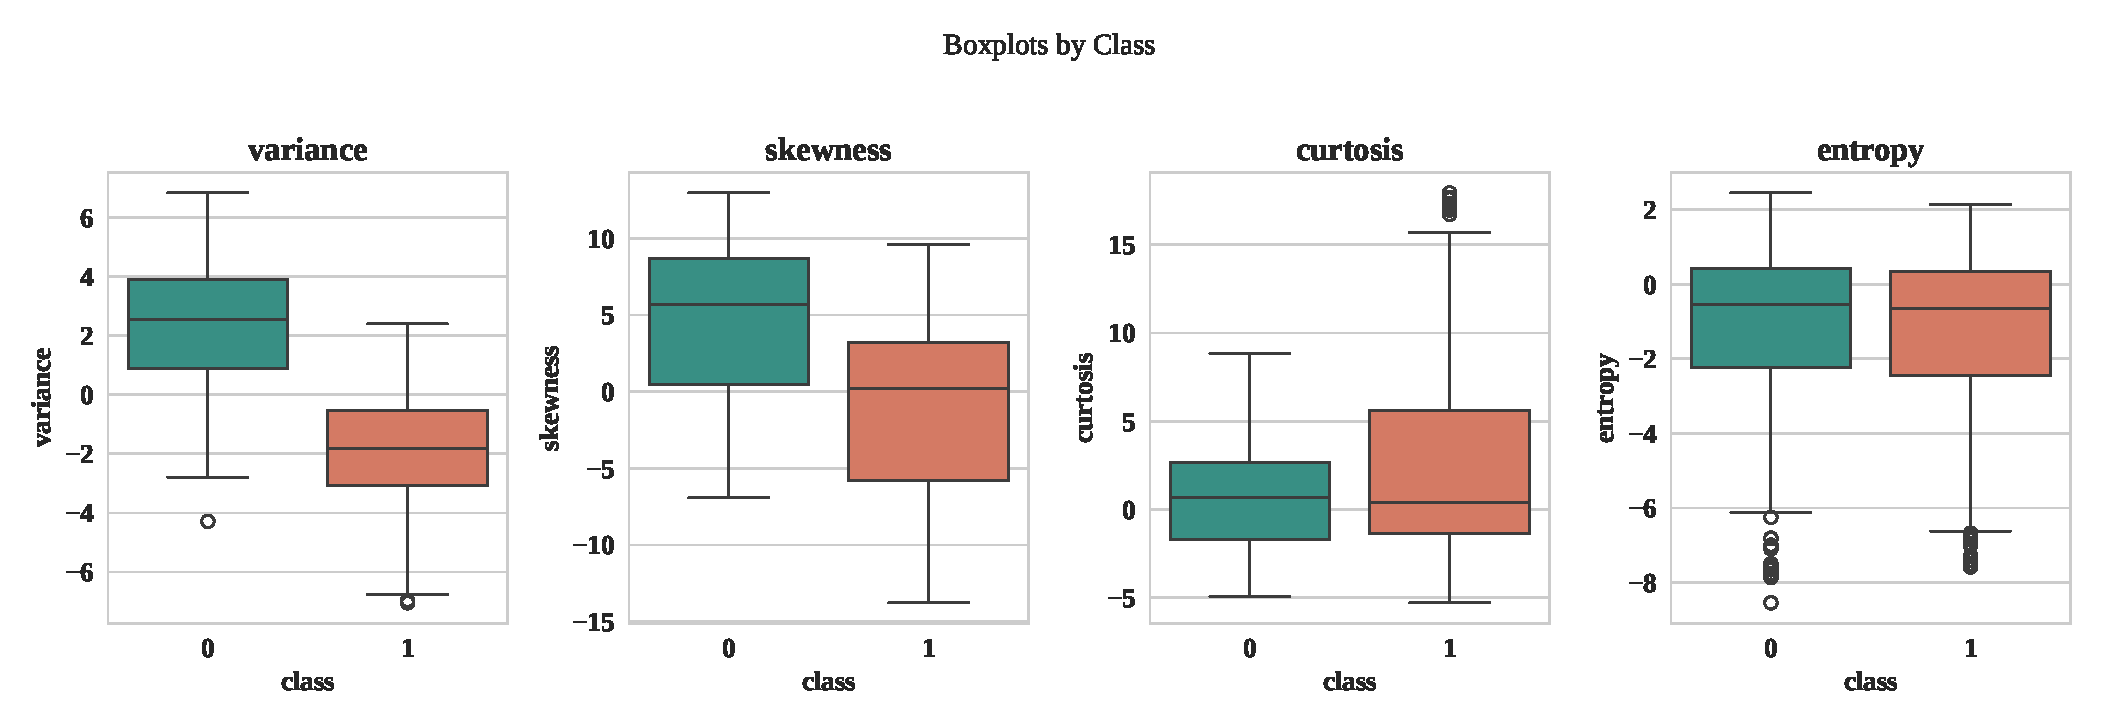
\includegraphics[width=0.95\textwidth]{figures/task2_boxplots.eps}
\caption{Boxplots of each feature by class.}
\end{figure}

Variance and skewness boxplots show minimal overlap in interquartile ranges between classes and the medians are clearly separated. Curtosis shows moderate separation and multiple outliers on authentic notes. Entropy's boxes almost completely overlap, consistent with its poor correlation earlier.

\subsection*{8.5 Training Error vs Epoch}
\begin{figure}[H]
\centering
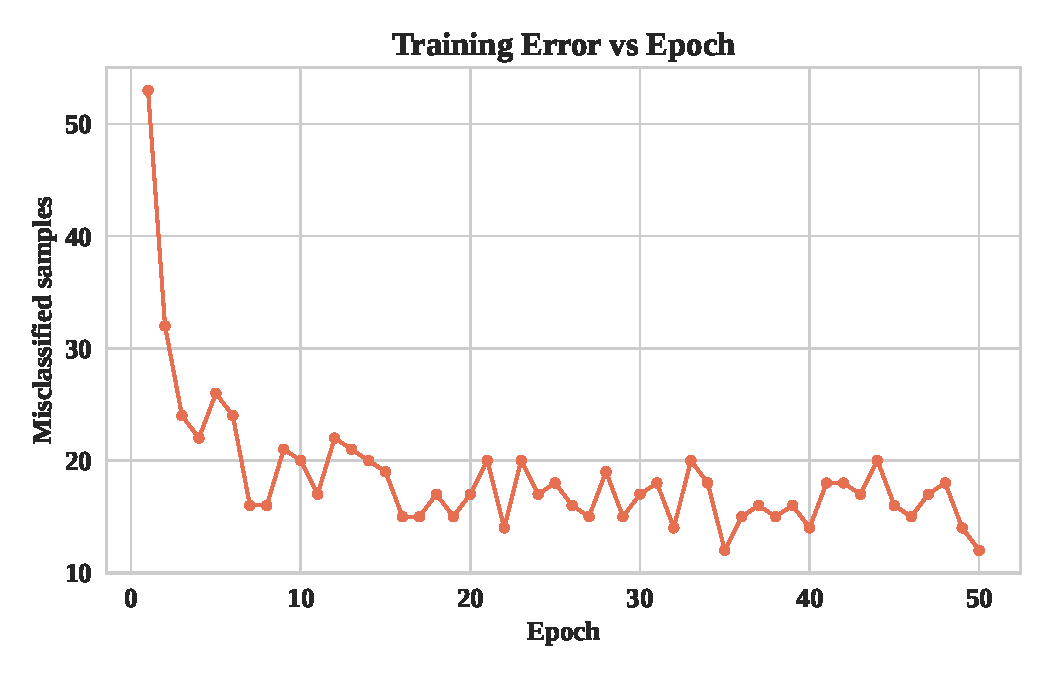
\includegraphics[width=0.7\textwidth]{figures/training_error_vs_epoch.eps}
\caption{Number of misclassified training samples per epoch.}
\end{figure}

Misclassification count drops sharply within the first several epochs, then stabilizes and slightly declines. It started at 53 misclassified samples and ended at just 12. It could not reach further optimization as the data is non-linearly separable.

\subsection*{8.6 Weight Evolution}
\begin{figure}[H]
\centering
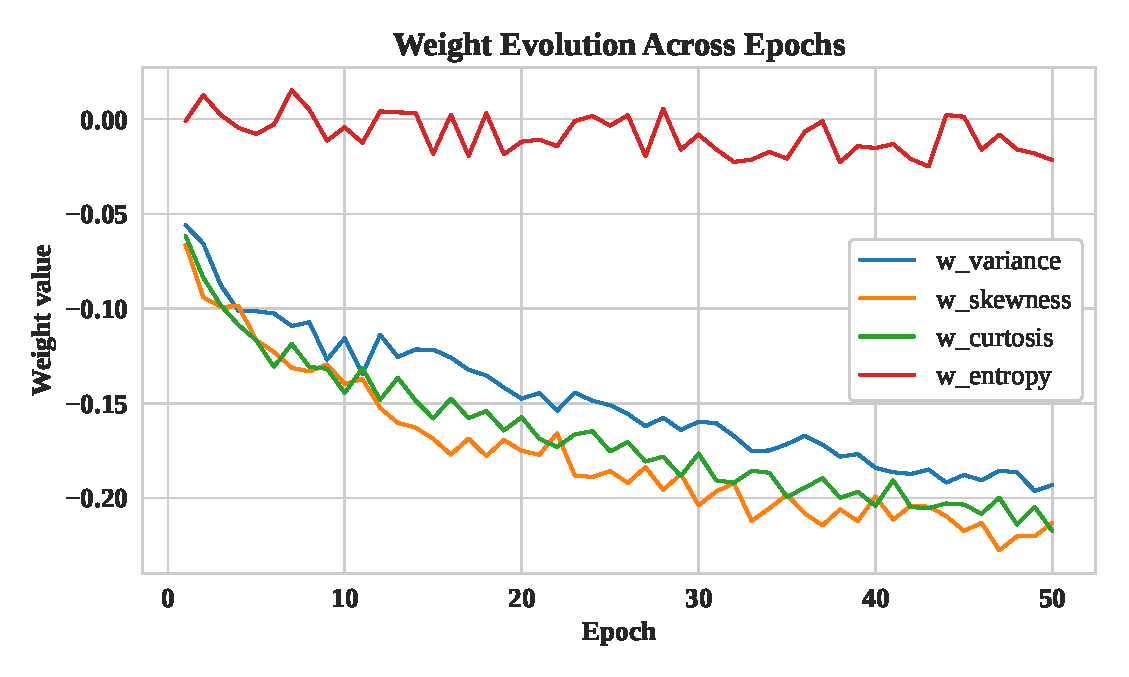
\includegraphics[width=0.7\textwidth]{figures/weight_evolution.eps}
\caption{Evolution of the four feature weights across training epochs.}
\end{figure}

Weights of variance, skewness and curtosis move further from their small random initial values and grow steadily in magnitude. The weight for entropy stays closest to zero throughout, since its correlation is very low with target class. By epoch 50 the final weight vector was $[-0.1931,\ -0.2132,\ -0.2176,\ -0.0217]$.

\subsection*{8.7 Bias Evolution}
\begin{figure}[H]
\centering
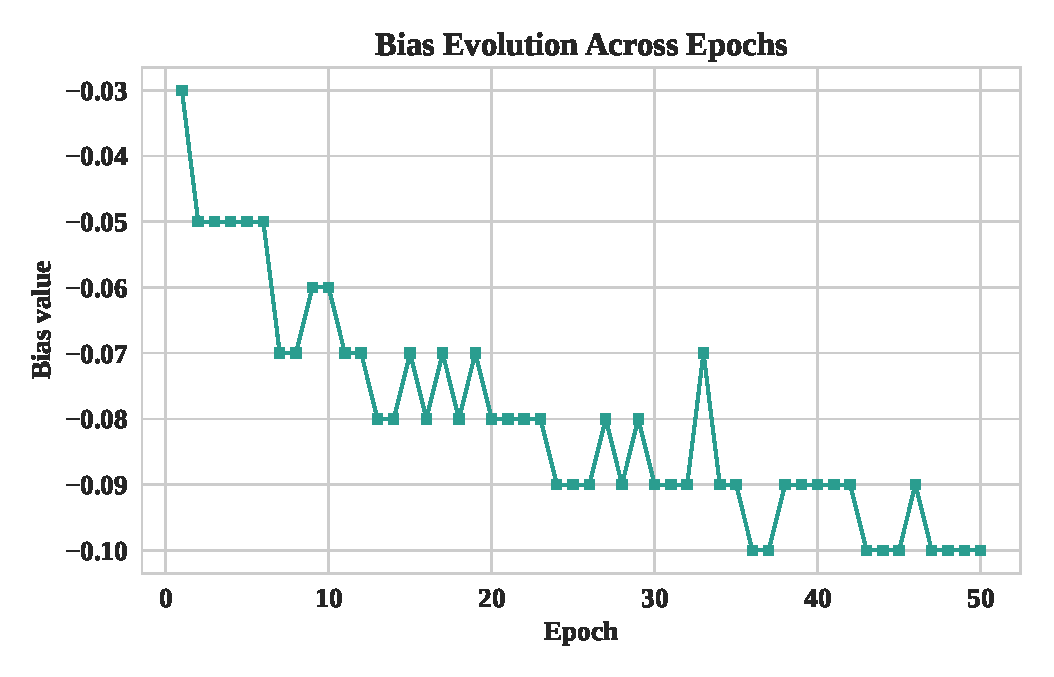
\includegraphics[width=0.7\textwidth]{figures/bias_evolution.eps}
\caption{Evolution of the bias term across training epochs.}
\end{figure}

The bias term shifts steadily downward during training, from $0$ initially to $-0.10$ by epoch 50, translating the decision hyperplane to better separate the two classes.

\subsection*{8.8 Confusion Matrix}
\begin{figure}[H]
\centering
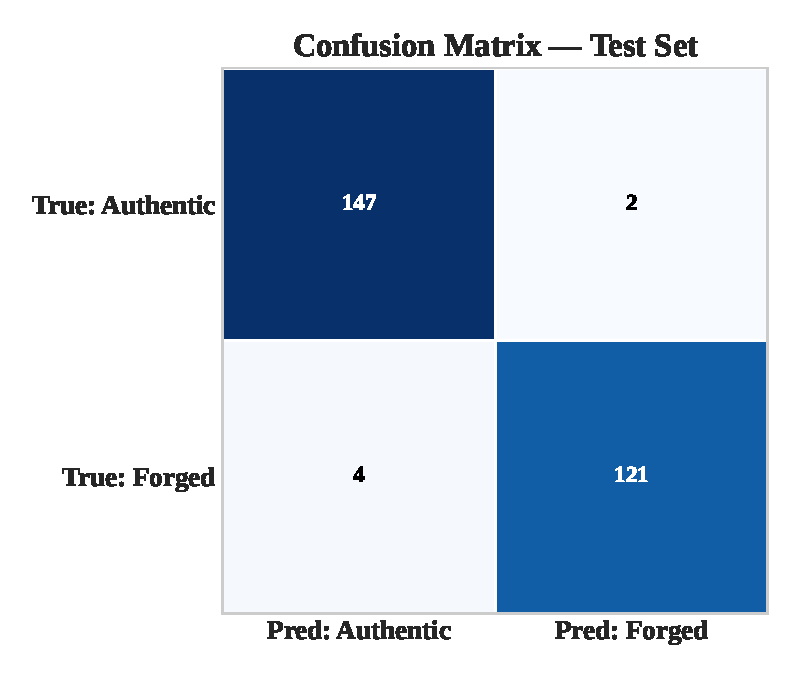
\includegraphics[width=0.55\textwidth]{figures/task6_confusion_matrix.eps}
\caption{Confusion matrix on the held-out test set.}
\end{figure}

The model correctly classifies the large majority of test samples (TP $=121$, TN $=147$), with only 2 FP and 4 FN. These errors tend to be in the overlapping region of variance and skewness.

\subsection*{8.9 Learning Rate Comparison}
\begin{figure}[H]
\centering
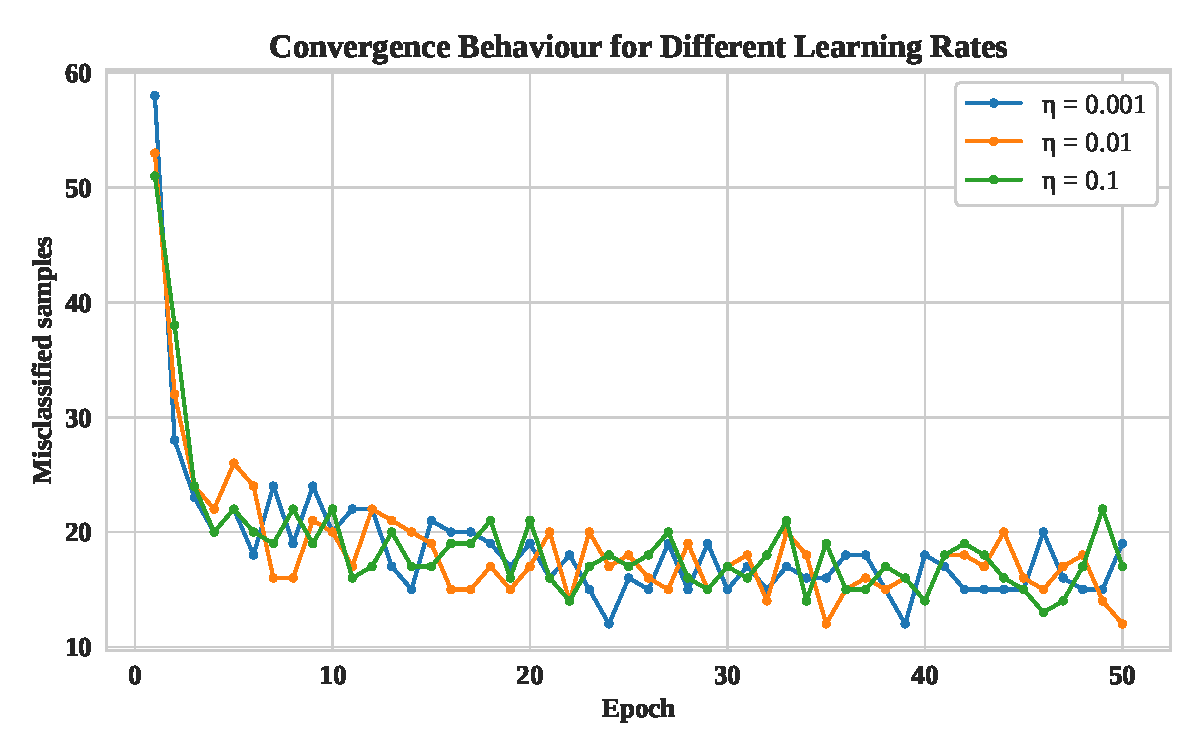
\includegraphics[width=0.7\textwidth]{figures/learning_rate_comparison.eps}
\caption{Convergence behaviour for $\eta \in \{0.001, 0.01, 0.1\}$.}
\end{figure}

 $\eta = 0.001$ converges slowly and smoothly, taking many more epochs to reach a low error count. $\eta = 0.01$ balances speed and stability well. $\eta = 0.1$ converges fastest initially but shows more oscillation between epochs, since each weight update is larger and can overshoot the ideal boundary -- a classic large-learning-rate trade-off.

\subsection*{8.10 Decision Boundary}
\begin{figure}[H]
\centering
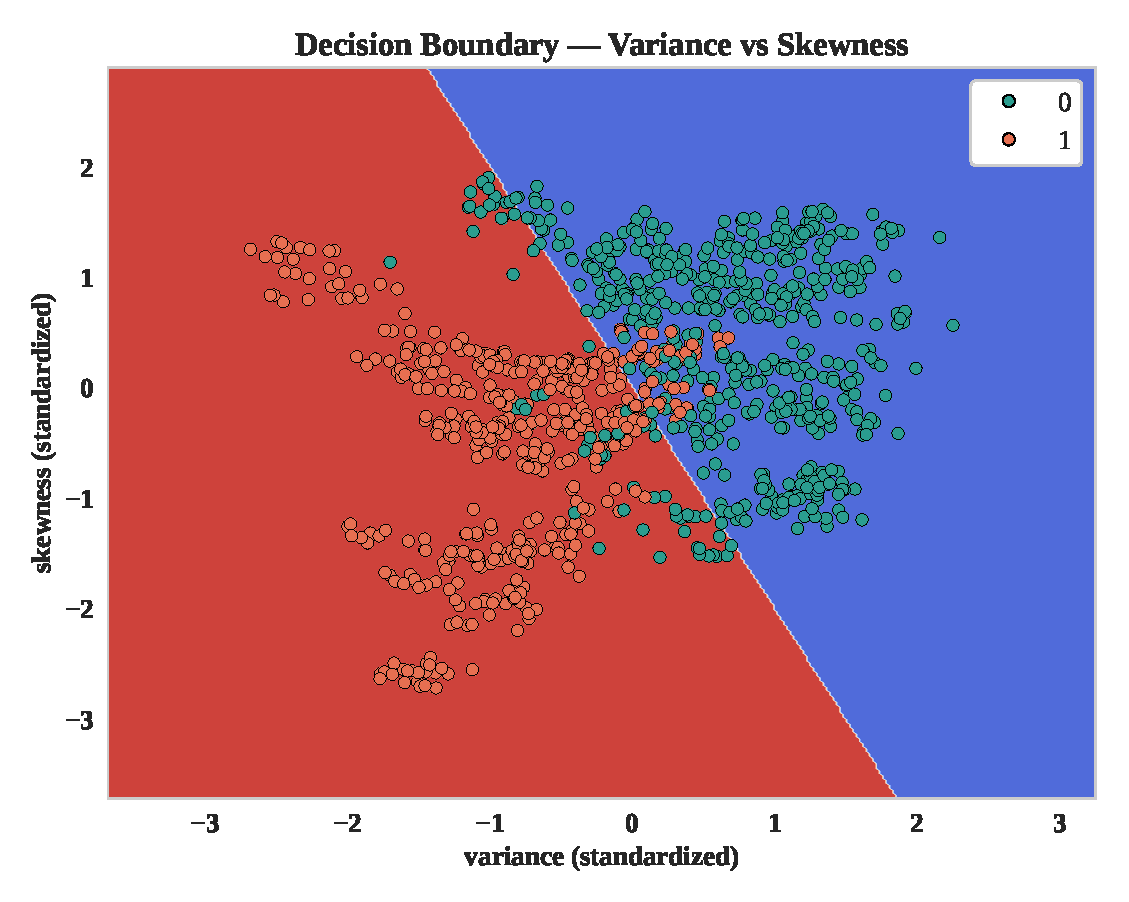
\includegraphics[width=0.65\textwidth]{figures/decision_boundary.eps}
\caption{Decision boundary using variance and skewness only.}
\end{figure}

The shaded regions show the linear boundary the 2-feature perceptron has learned. Most points fall on the correct side of the line, but the visible misclassifications near the boundary show that the two classes are non-linearly separable using only these two features.

%----------------------------------------------------------

\section*{9. Performance Tables}

\textbf{Training Summary}

\begin{tabular}{|p{6cm}|p{7cm}|}
\hline
Dataset Size & 1372 (1097 train / 275 test)\\
\hline
Train/Test Split & 80\% / 20\%\\
\hline
Learning Rate & 0.01\\
\hline
Epochs & 50 (ran to maximum; did not reach zero training error)\\
\hline
Final Weights & $[-0.1931,\ -0.2132,\ -0.2176,\ -0.0217]$\\
\hline
Final Bias & $-0.1000$\\
\hline
Accuracy & 0.9781\\
\hline
Precision & 0.9837\\
\hline
Recall & 0.9680\\
\hline
F1-score & 0.9758\\
\hline
\end{tabular}

\vspace{10mm}
\textbf{Confusion Matrix (Test Set)}

\begin{tabular}{|l|c|c|}
\hline
 & \textbf{Predicted Authentic} & \textbf{Predicted Forged}\\
\hline
\textbf{Actual Authentic} & TN = 147 & FP = 2\\
\hline
\textbf{Actual Forged} & FN = 4 & TP = 121\\
\hline
\end{tabular}

\vspace{10mm}

\textbf{Epoch-wise Learning (selected epochs)}

\begin{tabular}{|c|c|c|c|}
\hline
Epoch & Errors & Bias & $\lVert \mathbf{w} \rVert$\\
\hline
1  & 53 & $-0.0300$ & 0.1064\\
\hline
2  & 32 & $-0.0500$ & 0.1425\\
\hline
3  & 24 & $-0.0500$ & 0.1650\\
\hline
4  & 22 & $-0.0500$ & 0.1785\\
\hline
5  & 26 & $-0.0500$ & 0.1941\\
\hline
10 & 20 & $-0.0600$ & 0.2321\\
\hline
20 & 17 & $-0.0800$ & 0.2782\\
\hline
30 & 17 & $-0.0900$ & 0.3136\\
\hline
40 & 14 & $-0.0900$ & 0.3399\\
\hline
50 & 12 & $-0.1000$ & 0.3613\\
\hline
\end{tabular}

\vspace{10mm}

\textbf{Scikit-learn Comparison}

\begin{tabular}{|l|c|c|}
\hline
\textbf{Metric} & \textbf{Custom RosenblattUnit} & \textbf{sklearn.Perceptron}\\
\hline
Accuracy  & 0.9781 & 0.9781\\
\hline
Precision & 0.9837 & 0.9760\\
\hline
Recall    & 0.9680 & 0.9760\\
\hline
F1-score  & 0.9758 & 0.9760\\
\hline
\end{tabular}

%----------------------------------------------------------

\section*{10. Additional Tasks}

\subsection*{10.1 Step vs Sigmoid Activation}

\begin{figure}[H]
\centering
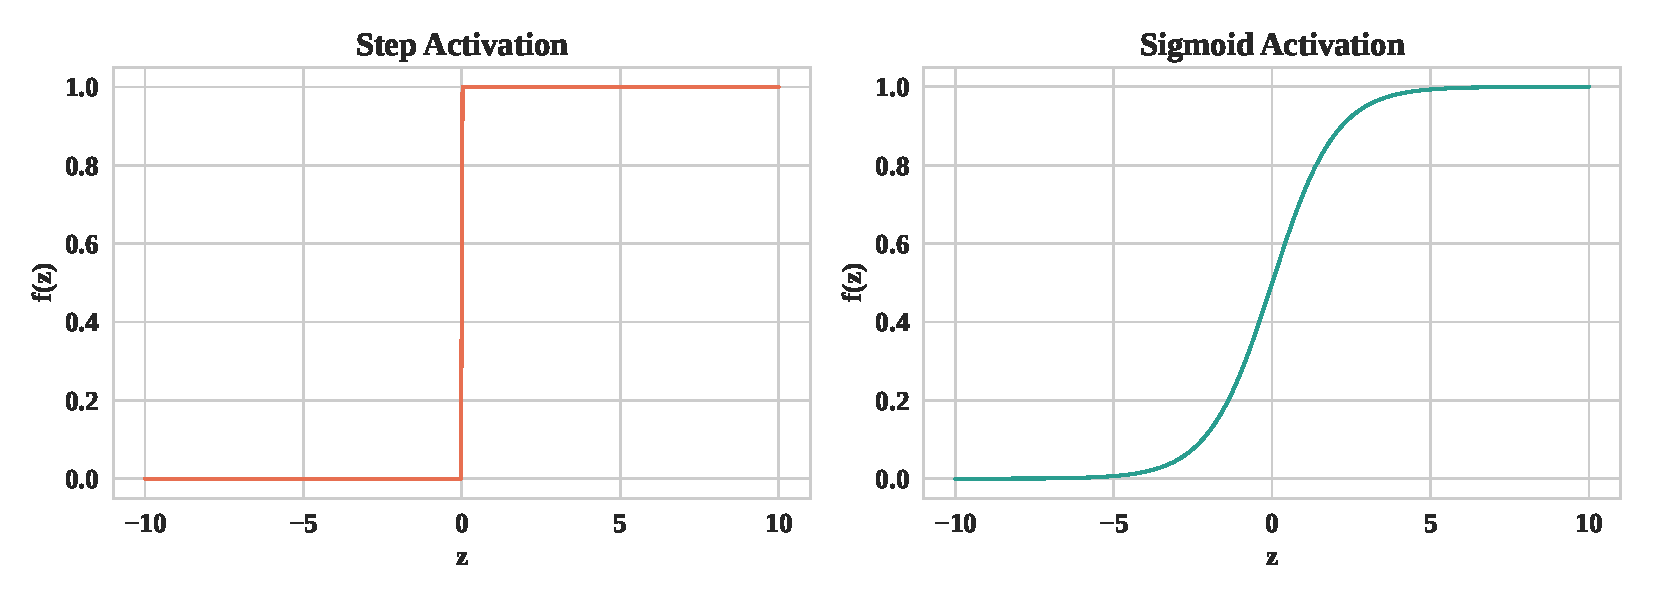
\includegraphics[width=0.85\textwidth]{figures/step_vs_sigmoid_activation.eps}
\caption{Step activation (left) vs.\ Sigmoid activation (right).}
\end{figure}
 The step function shows a discontinuity at $z=0$,  flat at $0$ till that and an instant jump to $1$, with zero gradient everywhere except that single undefined point. The sigmoid curve is smooth and continuous across the same range, with a non-zero gradient throughout most of its domain.


\subsection*{10.2 Comparison with Scikit-learn's Perceptron}

Both implementations achieve identical test accuracy (0.9781). The custom implementation has marginally higher precision (0.9837 vs.\ 0.9760) but slightly lower recall (0.9680 vs.\ 0.9760) than built-in perceptron, which makes the F1 score identical almost. This indicates that manual implementation is correct, with marginal variation with results.

\subsection*{10.3 Learning Rate Comparison}

Learning rates of 0.001, 0.01, 0.1 were tested. Lower learning rates converge more slowly but smoothly, while higher learning rates converge faster initially but oscillate more. These oscillations are caused because sample wise decision boundaries are large, and will overshoot the decision boundary.

\subsection*{10.4 Why a Single Layer Perceptron Cannot Solve XOR}

\begin{figure}[H]
\centering
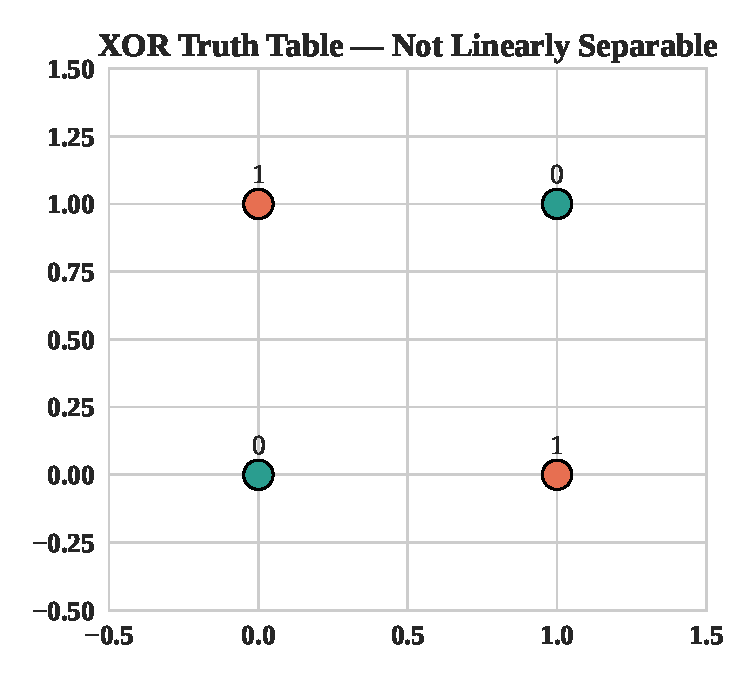
\includegraphics[width=0.5\textwidth]{figures/xor_not_linearly_separable.eps}
\caption{XOR truth table -- not linearly separable.}
\end{figure}

The four XOR points form two classes positioned at diagonally opposite corners of the square. No single straight line can separate the two colors without misclassifying at least one point. This shows why sinlge layer perceptron cannot solve XOR problem, as there is no linear separability.

\subsection*{10.5 Effect of Feature Normalization on Convergence}

\begin{figure}[H]
\centering
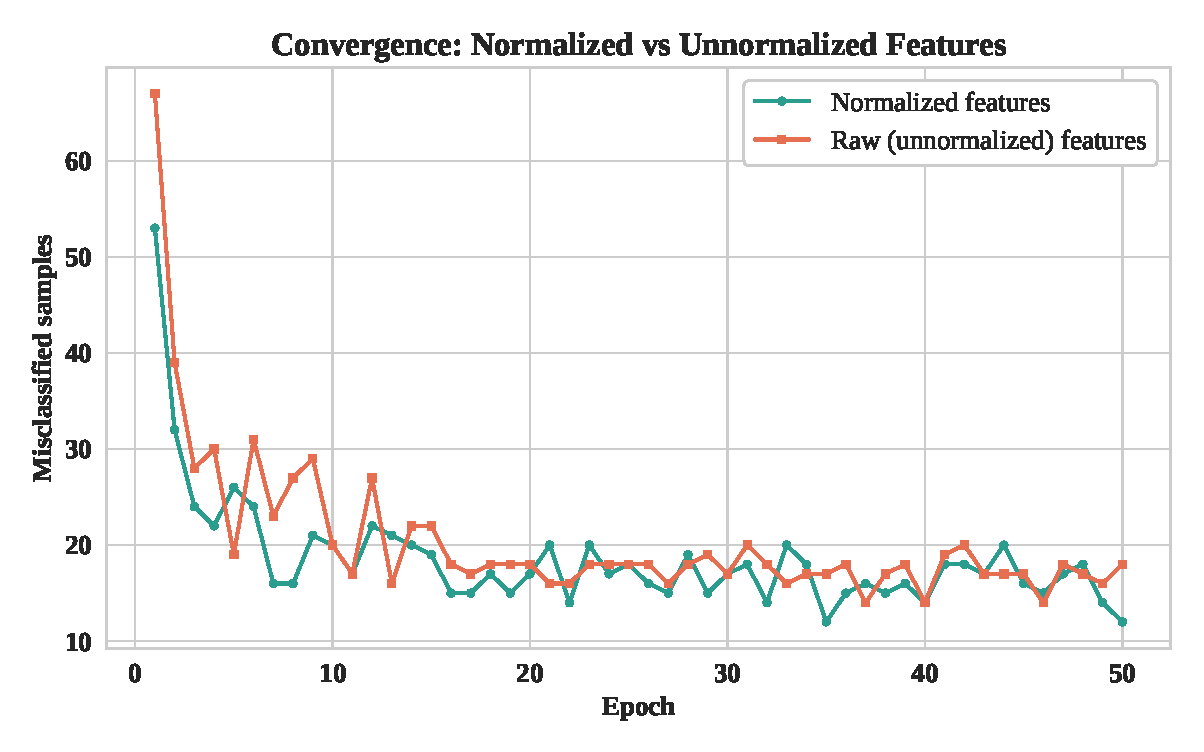
\includegraphics[width=0.7\textwidth]{figures/normalization_effect_on_convergence.eps}
\caption{Convergence comparison: normalized vs.\ unnormalized features.}
\end{figure}
The normalized-feature curve converges faster and more smoothly than the unnormalized curve. Without normalization, features with larger natural numeric ranges like skewness, curtosis dominate the weight updates, slowing convergence and causing more erratic error counts across epochs.

%----------------------------------------------------------

%----------------------------------------------------------

\section*{11. Additional Experiment}

The perceptron learning algorithm was implemented independently for three fundamental logic gates (AND, OR, NOT ) for 2 bit data to observe how a single layer perceptron learns different linearly separable boolean functions. Weights and biases were initialized as 0 for every gate, and the perceptron weight update algorithm was applied., and decision boundaries were plotted after the model converges. This experiment proves that single layer perceptron work well on linearly separable data, as there are no errors in the model post convergence and the model has classified all data points correctly.\\

\begin{figure}[H]
\centering
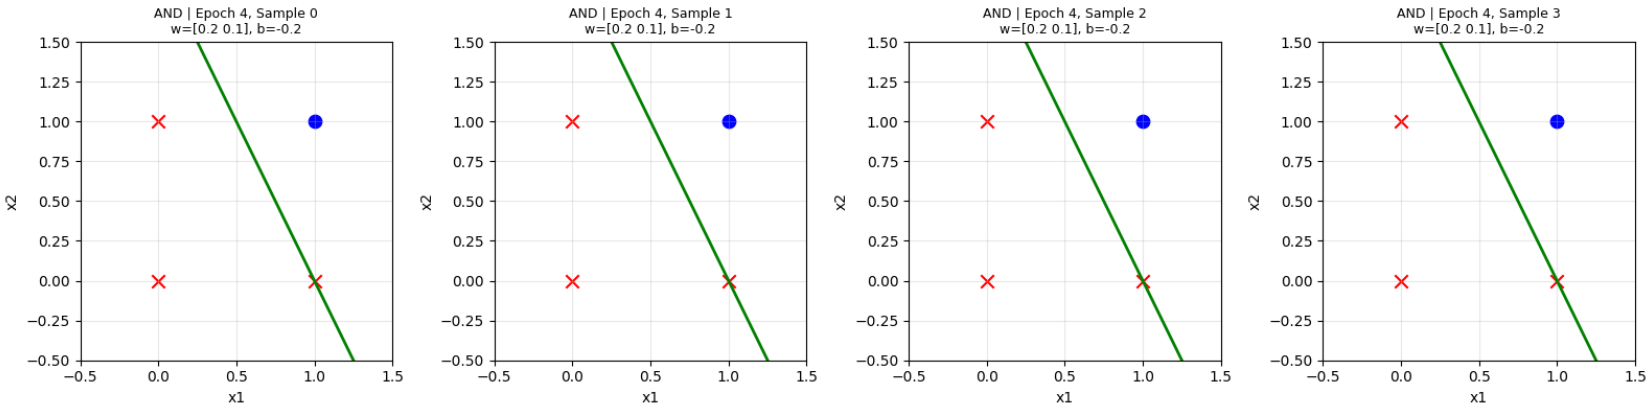
\includegraphics[width=1\textwidth]{figures/and.png}
\caption{Decision boundary evolution for the AND gate.}
\end{figure}

\begin{figure}[H]
\centering
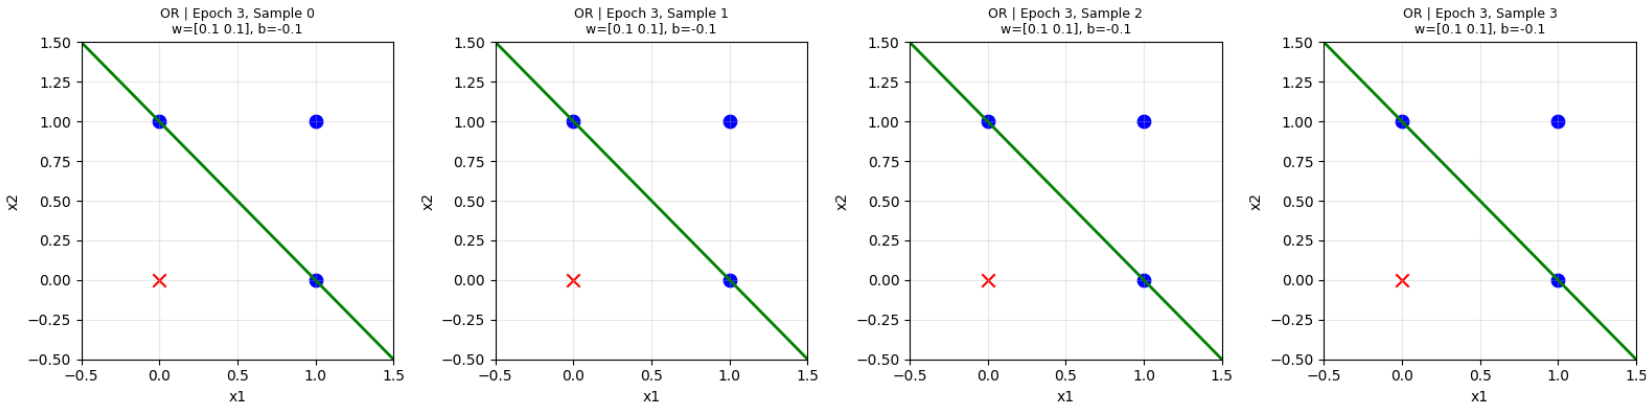
\includegraphics[width=1\textwidth]{figures/or.png}
\caption{Decision boundary evolution for the OR gate.}
\end{figure}

\begin{figure}[H]
\centering
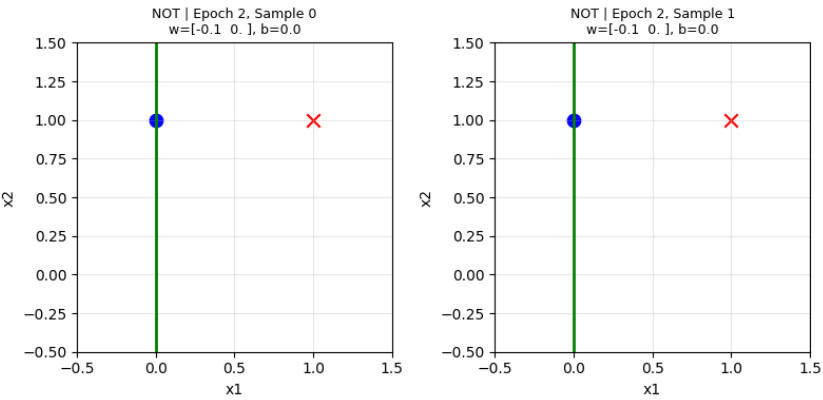
\includegraphics[width=0.7\textwidth]{figures/not.png}
\caption{Decision boundary evolution for the NOT gate.}
\end{figure}

\vspace{3mm}

\textbf{Initial and Final Weights/Bias Summary}

\begin{center}
\begin{tabular}{|l|c|c|c|c|c|}
\hline
\textbf{Gate} & \textbf{Initial Weights} & \textbf{Initial Bias} & \textbf{Final Weights} & \textbf{Final Bias} & \textbf{Epochs Taken}\\
\hline
AND & [0,0] & 0 & [0.2,0.1] & -0.2 & 4\\
\hline
OR  & [0,0] & 0 & [0.1,0.1] & -0.1 & 3\\
\hline
NOT & [0,0] & 0 & [-0.1,0] & 0 & 2\\
\hline
\end{tabular}
\end{center}

%----------------------------------------------------------
\section*{12. Discussion}

The single-layer perceptron, trained from scratch using Rosenblatt's original learning rule, achieved strong performance  (97.81\% test accuracy, F1-score 0.9758). This shows that the given features are highly discriminative between the two classes. Variance, skewness and curtosis contributed majorly in identifying the classes, while entropy had contributed the least.

The training-error curve shows the model did not reach zero misclassifications even after 50 epochs, and misclassified 12 data points on the training set. This indicates the classes are close to, but not perfectly linearly separable. A perceptron with a hard step activation cannot resolve this partial overlap even on training with more epochs, since it produces only a hyperplane as a decision boundary.

The learning rate study demonstrates bias-variance, i.e smaller $\eta$ gives smoother but slower convergence, while larger $\eta$ risks oscillation from overshooting the optimal decision boundary. The comparison against Scikit-learn's builtin perceptron proves the correctness of the manual implementation from scratch as both achieve only marginally different performance (caused by minor implementation differences).

The single layer perceptron was then tried on basic logic gates of AND, OR, NOT and XOR. The model was able to produce clear decision boundaries for linearly separable data like AND, OR and NOT gate. However, it could not produce proper decision boundaries which classifies all points correctly, as there is no possible linear boundary for the XOR problem. This additional experiment clearly points out the flaw in single layer perceptrons, which is the lack of ability to draw decision boundaries for non-linearly problems. This problem can be solved by multilayer perceptrons with hyperparameter tunings, to be studied on upcoming experiments.\\

%----------------------------------------------------------

\section*{13. Conclusion}

In this experiment, a Single Layer Perceptron was successfully implemented from scratch using NumPy and applied to the UCI Banknote Authentication dataset. The perceptron learning rule, step activation function, and weight and bias update mechanism were implemented manually. The trained model achieved 97.81\% accuracy, 98.37\% precision, 96.80\% recall, and an F1-score of 0.9758 on the test set, which is almost as same as the builtin perceptron implementation. 

The additional experiment demonstrated clearly how single layer perceptrons can solve only linearly separable problems, and why they sturggle with non-linearly separable datasets. Other additional tasks compared the efficiency of step and sigmoid activation functions, tested multiple learning rates to find optimal value,  and studied the effect of normalization on convergence.

%----------------------------------------------------------

\section*{14. References}

\begin{enumerate}
\item F. Rosenblatt, ``The Perceptron,'' \emph{Psychological Review}, 1958.
\item I. Goodfellow, Y. Bengio and A. Courville, \emph{Deep Learning}, MIT Press, 2016.
\item C. M. Bishop, \emph{Pattern Recognition and Machine Learning}, Springer, 2006.
\item S. Haykin, \emph{Neural Networks and Learning Machines}, Pearson, 2009.
\item UCI Machine Learning Repository -- Banknote Authentication Dataset.
\item Scikit-learn Documentation: Perceptron.
\end{enumerate}

%----------------------------------------------------------

\section*{15. Source Code}

The complete source code, generated outputs, and result tables for this experiment are available at the following GitHub repository:

\begin{center}
\url{https://github.com/Ashwin271206/dl-lab/tree/main/Lab%201}
\end{center}


\end{document}